%!TEX root = ../dissertation.tex

\chapter{Background}

%% FIGURE OUT HOW TO START HTIS CHAPTER HERE 
\newthought{There's something to be said} for having a good opening line. Morbi commodo, ipsum sed pharetra gravida, orci  $x = 1/\alpha$ magna rhoncus neque, id pulvinar odio lorem non turpis \cite{Eigen1971, Knuth1968}. 


\section{Causal Effects} 

A traditional understanding of causation comes from the field of medicine, where researchers can perform a controlled experiment to prove causation.  This type of study contains two sample groups, one which receives no treatment (the placebo group) and one which receives the treatment (the treatment group).  By comparing the outcome of these two groups, the researchers can demonstrate whether the outcome for patients receiving treatment differs significantly from the controls.  

To translate this idea into statistical terms, some notation must be introduced.  The random variable $A$ represents the treatment status, where a value of 1 indicates treated and a value of 0 indicates untreated.  The random variable $Y$ is the outcome variable, often with a value of 0 indicating survival and a value of 1 indicating death.  These interpretations of $A$ and $Y$ correspond to the above understanding of causation studies, but for various causal inference studies, the form of $Y$ and  in particular can change depending on the question of interest.  For example, $Y$ can be a continuous variable, such as the weight difference of an individual in a weight loss trial or the change in HDL levels in a cholesterol study. 

To study the causal effect of $A$, the desired value is the difference in $Y$ under the varying conditions of $A$.  Notationally, this is the difference between $Y^{\, a=1}$, the outcome under treatment, and $Y^{\, a=0}$, the outcome under no treatment.  A causal effect can be seen on an individual level if $\; Y_i^{\, a=1} \neq Y_i^{\, a=0}$ for individual $i$.  By considering how each individual's responses to varying treatments differ, causation (or lack thereof) can easily be determined using paired differences of the form 
$$\; Y_i^{\, a=1} - Y_i^{\, a=0}$$ 
These differences would be tested against the null hypothesis of zero difference in outcome for varying treatments.  

However, certain difficulties arise using this method.  In many studies, it is impossible to have scenarios of both treatment and no treatment for the same individual, particularly if a potential outcome is death.  Typically, individuals either have $\; Y_i^{\, a=1}$ or  $Y_i^{\, a=0}$, but not both, making it impossible to calculate the paired differences.  Therefore, a controlled double blinded experiment is often performed, where each individual is randomly assigned treatment or placebo.  In these studies, the statistic of interest is the average causal effect in the population, 
$$ \mathbb{E}[Y^{\; a=1}] - \mathbb{E}[Y^{\; a=0}]$$ 
Mathematically, this is equivalent to 
$$ \mathbb{E}[Y^{\; a=1} - Y^{\; a=0}]$$ 
because the average of differences is equal to the difference of averages \cite{hernan_robins_2016}.  Note, that this is not the same as calculating the mean of paired differences as if each individual had received both treatments at different times to calculate individual causal effects.  Rather, the difference in the means of the placebo and treatment groups is being calculated to estimate average causal effect across the population.  

\subsection{IP Weighting} 
Many of the concerns discussed above can by addressed using the method of IP weighting, which simulated a psuedo-population in which every individual has two data inputs, that of treatment and that of no treatment.  The method by which this is done is by considering a covariate of the data, $L$, another value which is known before treatment is assigned.  The idea of conditional exchangeability can be used to see that $Y^{a} \Perp A\mid L$ in the original population because $A$ is independent of $L$ \cite{hernan_robins_2016}.  The pseudo-population can be calculated with the following for each of the possible $A$ and $L$ combinations 
$$ n\cdot Pr[Y=y \mid A = a, L= 1] \cdot Pr[A=a \mid L=l]  \cdot Pr[L=l] \cdot \frac{1}{Pr[A = a \mid L = 1]} $$ 
where the last term here is the IP weight.  This form can be used to solve for the standardized mean as follows, 
\begin{align} 
E[Y^{\,a}] &= \sum_l n \cdot Pr[Y=y \mid A = a, L= 1] \cdot Pr[A=a \mid L=l]  \cdot Pr[L=l] \cdot \frac{1}{Pr[A = a \mid L = 1]} \\ 
&=  \sum_l n \cdot Pr[Y=y \mid A = a, L= 1] \cdot Pr[L=l]\\ 
&= \sum_l E[Y \mid A=a, L= l] Pr[L=l] 
\end{align} 


\subsection{Assumptions} 
% Cox (1958) -- independence of observations 
% Rubin 1980 
% no multiple versions of treatment in STUVA 
% check textbook page 5 
%- SUTVA: http://www2.stat.duke.edu/courses/Spring14/sta320.01/Class2.pdf




\section{Parametric G-formula} 

\section{G-estimation} 

\section{Doubly Robust Estimation} 


% For an example of a full page figure, see Fig.~\ref{fig:myFullPageFigure}.


%\begin{figure}
%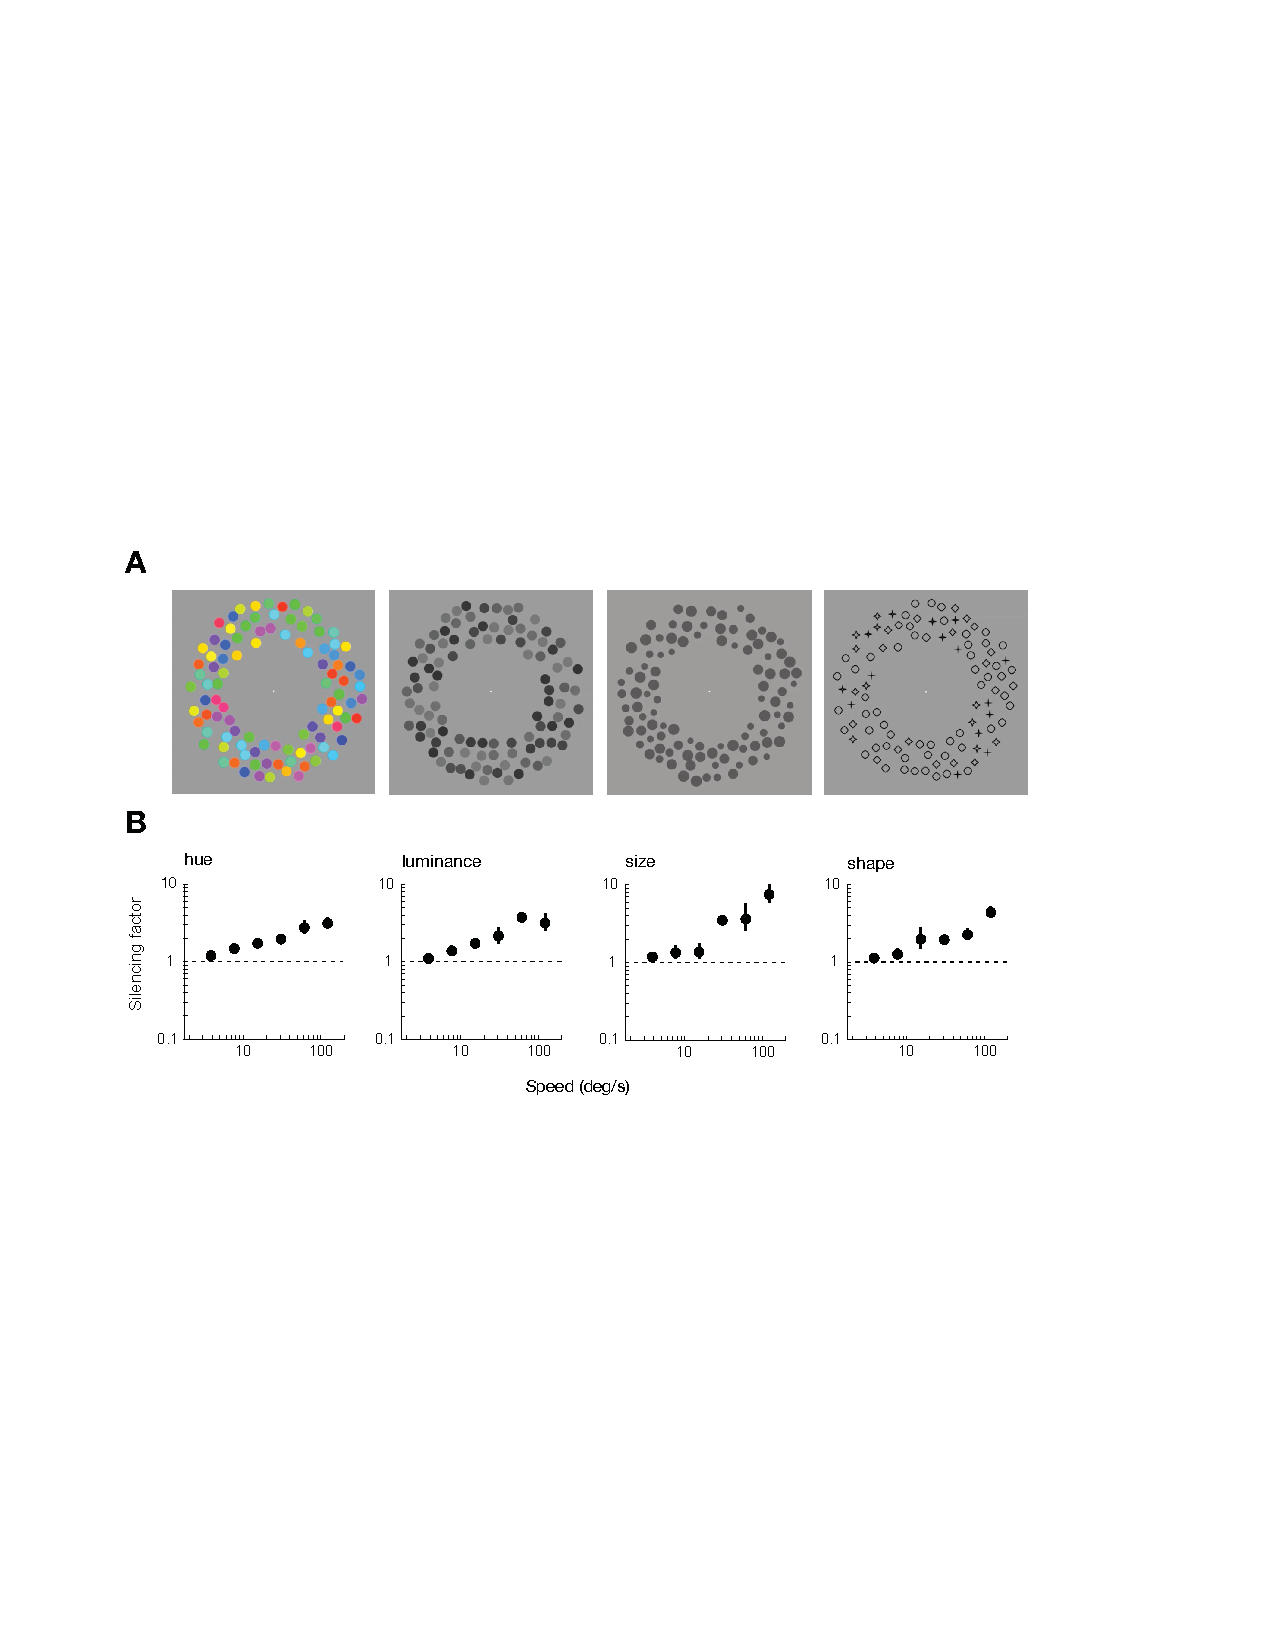
\includegraphics[width=\textwidth]{figures/fig1}
%\caption[Short figure name.]{This is a figure that floats inline and here is its caption.
%\label{fig:myInlineFigure}}
%\end{figure}
